\documentclass[spanish,aspectratio=169,10pt]{beamer}
\usepackage[utf8]{inputenc}
\usepackage[T1]{fontenc}
\usepackage[spanish,es-tabla]{babel}
\usepackage[scaled=.96]{helvet}
\renewcommand{\familydefault}{\sfdefault}
\usepackage{booktabs}
\usepackage{tabularx}
\usepackage{tikz}
\usepackage{hyperref}
\usetikzlibrary{positioning,shapes.geometric}

\definecolor{unadmDark}{HTML}{174A3A}
\definecolor{unadmGreen}{HTML}{5F8F3A}
\definecolor{unadmGold}{HTML}{B88A2A}
\definecolor{paper}{HTML}{F6F7F2}
\definecolor{ink}{HTML}{1F2A24}
\setbeamercolor{normal text}{fg=ink,bg=white}
\setbeamercolor{structure}{fg=unadmGreen}
\setbeamercolor{frametitle}{fg=white,bg=unadmDark}
\setbeamercolor{block title}{fg=white,bg=unadmGreen}
\setbeamercolor{block body}{fg=ink,bg=paper}
\setbeamertemplate{navigation symbols}{}
\setbeamertemplate{itemize item}{\color{unadmGold}$\blacktriangleright$}
\setbeamertemplate{footline}{%
  \leavevmode\hbox{%
  \begin{beamercolorbox}[wd=.71\paperwidth,ht=2.5ex,dp=1ex,leftskip=1em]{author in head/foot}\color{white}\bfseries Interaprendizaje en ambientes virtuales\end{beamercolorbox}%
  \begin{beamercolorbox}[wd=.29\paperwidth,ht=2.5ex,dp=1ex,rightskip=1em plus1fil]{date in head/foot}\color{white}Actividad 7\hfill\insertframenumber/\inserttotalframenumber\end{beamercolorbox}}
}
\setbeamercolor{author in head/foot}{bg=unadmDark}
\setbeamercolor{date in head/foot}{bg=unadmGreen}
\hypersetup{colorlinks=true,urlcolor=unadmGreen}

\title{Lex Digital Unipersonal}
\subtitle{Brief profesional y prototipo de despacho jurídico virtual}
\author{Martin Jonathan de la Cruz · ES2611202040}
\institute{Universidad Abierta y a Distancia de México\\Licenciatura en Derecho · Semestre 2, Bloque 1\\Figura docente: Janeth Santana Ramírez}
\date{Actualización técnica: 26 de agosto de 2026}

\begin{document}

\begin{frame}[plain]
\begin{tikzpicture}[remember picture,overlay]
  \fill[unadmDark] (current page.south west) rectangle ([xshift=.61\paperwidth]current page.north west);
  \fill[unadmGreen] ([xshift=.61\paperwidth]current page.south west) rectangle (current page.north east);
  \node[circle,draw=unadmGold,line width=2pt,minimum size=2.8cm,text width=2.2cm,align=center,text=white,font=\bfseries] at ([xshift=-3.6cm,yshift=-2.8cm]current page.north east) {LEX\\DIGITAL};
  \node[rounded corners,fill=unadmGold,text=white,font=\scriptsize\bfseries,inner xsep=7pt,inner ysep=4pt] at ([xshift=-3.6cm,yshift=-4.65cm]current page.north east) {PROTOTIPO ALFA 0.5.0};
\end{tikzpicture}
\vspace{1.05cm}
\begin{minipage}{.56\textwidth}
{\color{white}\LARGE\bfseries Lex Digital Unipersonal\par}
\vspace{.28cm}{\color{unadmGold}\rule{7.8cm}{1.3pt}}\vspace{.28cm}
{\color{white}\large Atención jurídica digital clara, protegida y verificable\par}
\vspace{.55cm}{\color{white}\large Martin Jonathan de la Cruz\par}
{\color{white!80}\small Matrícula ES2611202040\\Brief profesional · Actividad 7 · 26 de agosto de 2026}
\end{minipage}
\end{frame}

\begin{frame}{Identidad, propósito y servicios}
\small
\begin{columns}[T,onlytextwidth]
\column{.48\textwidth}
\begin{block}{Propósito}
Acompañar asuntos jurídicos en entornos digitales mediante comunicación comprensible, fuentes verificadas y protección responsable de la información.
\end{block}
\textbf{Servicios propuestos}
\begin{itemize}
  \item orientación y análisis jurídico inicial;
  \item organización documental por asunto;
  \item investigación de fuentes oficiales;
  \item seguimiento y comunicación intercultural.
\end{itemize}
\column{.48\textwidth}
\begin{block}{Valor para la persona usuaria}
Un solo espacio para conocer el estado del asunto, revisar acuerdos y conservar versiones identificables, siempre con revisión humana antes de entregar.
\end{block}
\textbf{Especialización digital:} privacidad, evidencia electrónica y uso ético de tecnología e IA.
\end{columns}
\vspace{2pt}
\alert{Alcance académico:} plataforma en desarrollo por el autor; las demostraciones utilizan exclusivamente información ficticia \cite{lexDigital2026}.
\end{frame}

\begin{frame}{Protocolo de ciberseguridad y confidencialidad}
\begin{columns}[T,onlytextwidth]
\column{.55\textwidth}
\centering
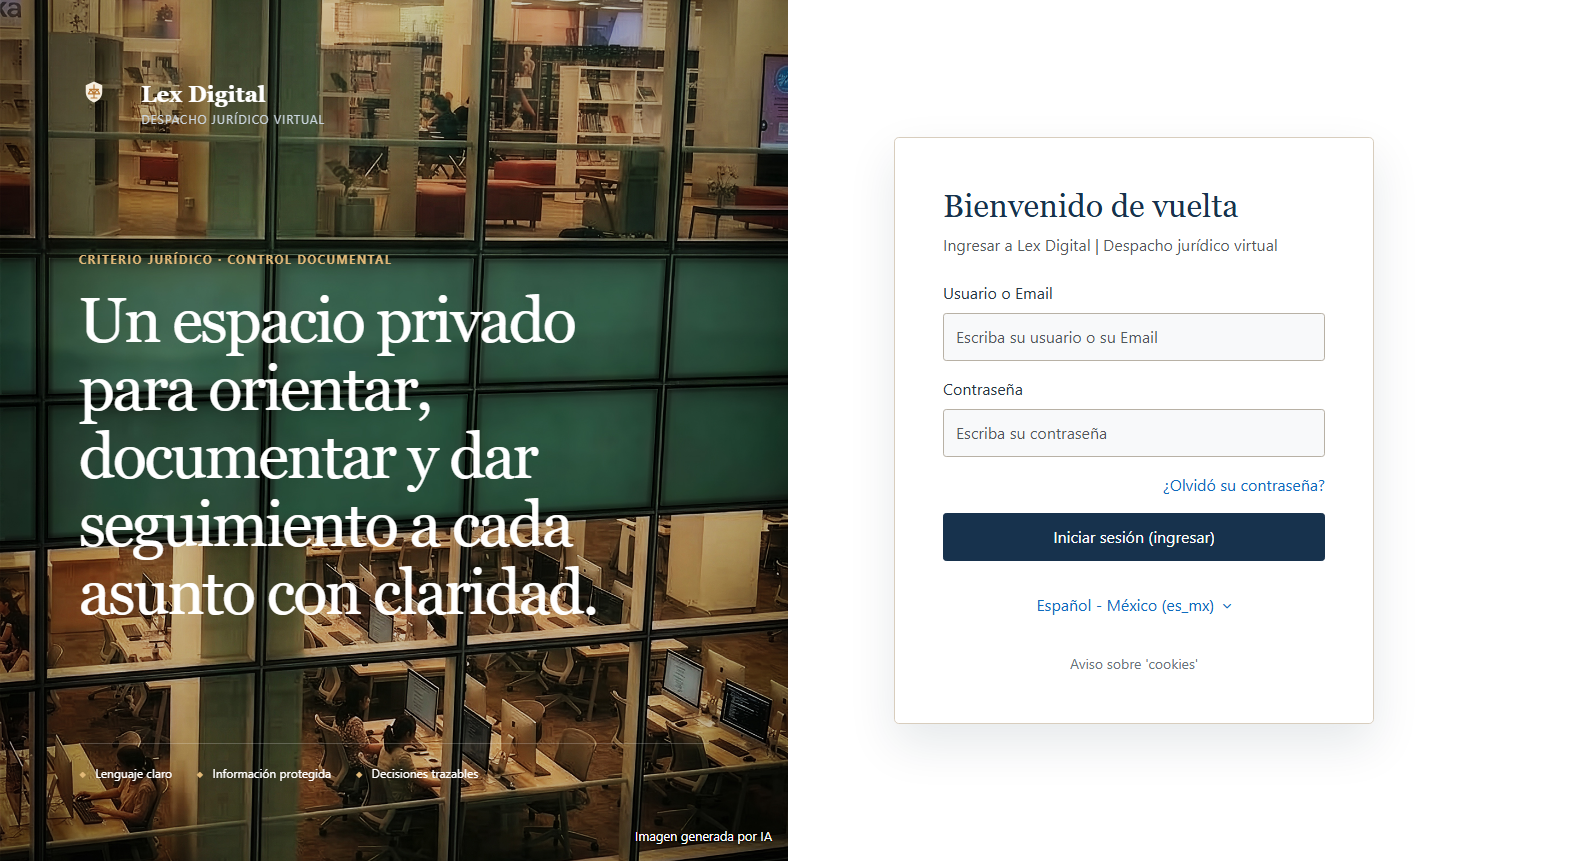
\includegraphics[width=\linewidth,height=.65\textheight,keepaspectratio]{img/actividad-7/lexdigital/01-login-publico.png}
\column{.42\textwidth}
\footnotesize
\begin{block}{Controles operativos}
\begin{itemize}
  \item \textbf{Acceso:} cuenta individual y permisos mínimos por asunto.
  \item \textbf{No difusión:} datos y documentos solo dentro del canal autorizado.
  \item \textbf{Repositorio:} una versión maestra con historial de cambios.
  \item \textbf{Respaldo:} copia cifrada y prueba de recuperación.
  \item \textbf{Incidentes:} contener, registrar, corregir y evaluar notificación.
  \item \textbf{IA:} no ingresar datos confidenciales y revisar toda salida.
\end{itemize}
\end{block}
\end{columns}
\vfill
{\scriptsize El protocolo aplica minimización, finalidad y control de acceso; no sustituye el análisis jurídico de cada caso \cite{camaraDiputados2025lfpdppp}.}
\end{frame}

\begin{frame}{Estructura funcional y responsabilidades}
\begin{columns}[T,onlytextwidth]
\column{.56\textwidth}
\centering
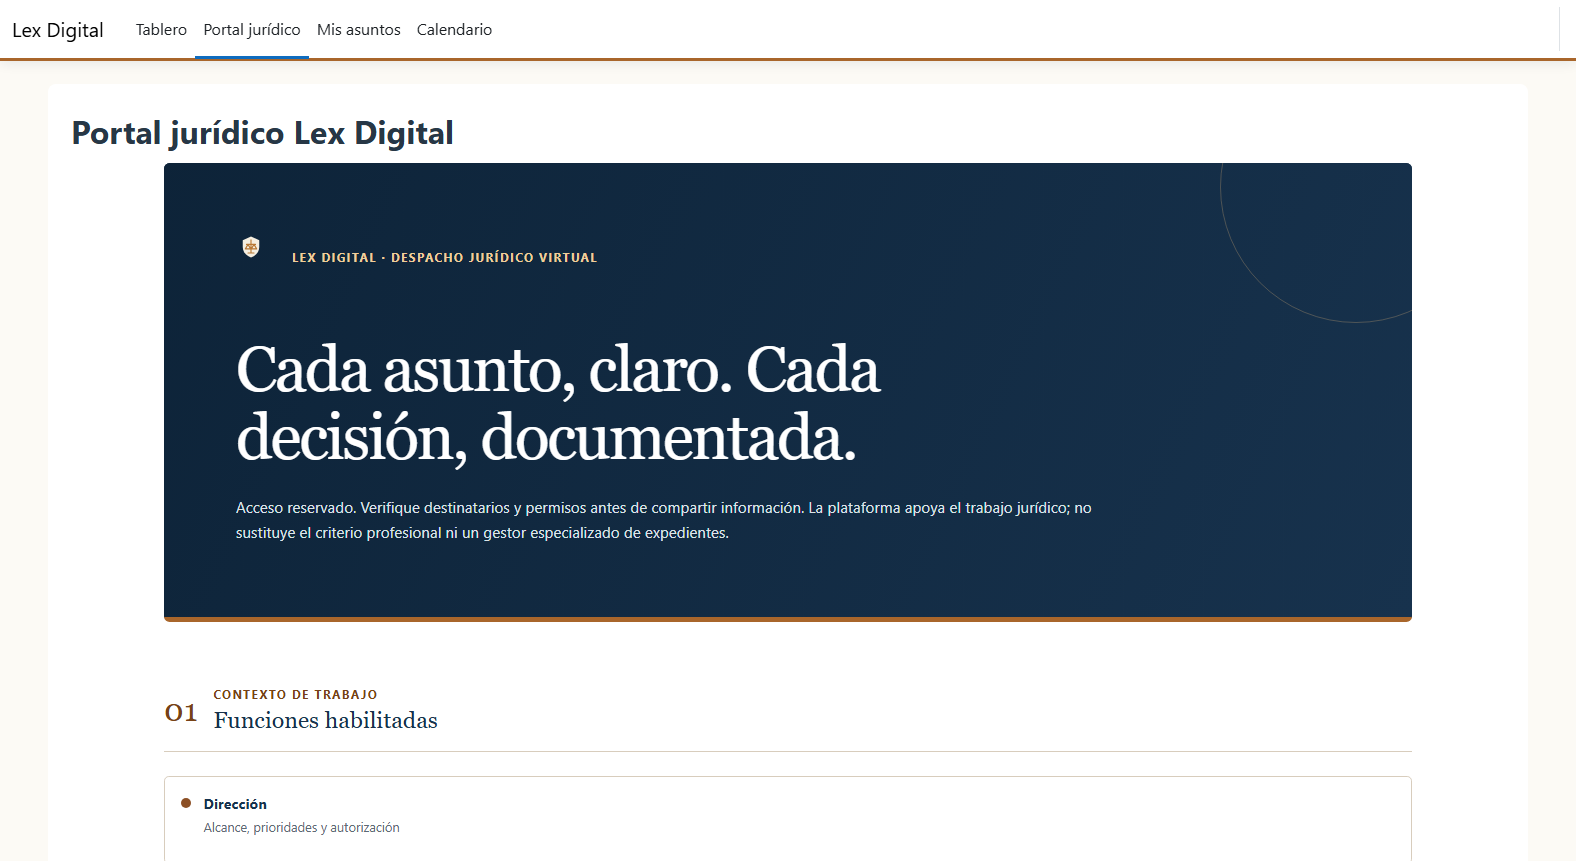
\includegraphics[width=\linewidth,height=.62\textheight,keepaspectratio]{img/actividad-7/lexdigital/02-portal-demo-direccion.png}
\column{.41\textwidth}
\scriptsize
\begin{tabularx}{\linewidth}{>{\bfseries}p{2.1cm}X}
\toprule
Función & Responsabilidad \\
\midrule
Dirección & Delimita alcance y autoriza cierre. \\
Investigación & Verifica hechos, normas y fuentes. \\
Redacción & Integra versiones y citas. \\
Atención & Registra acuerdos y comunica avances. \\
Calidad & Revisa fundamento, datos y permisos. \\
\bottomrule
\end{tabularx}
\vspace{3pt}
En la modalidad unipersonal, Martin Jonathan de la Cruz ejerce cada función en etapas separadas y deja evidencia del cambio de rol \cite{lopezMartinez2022trabajoCooperativo,conocer2025ec0554}.
\end{columns}
\vfill
{\scriptsize La separación funcional permite crecer sin perder responsabilidades ni trazabilidad.}
\end{frame}

\begin{frame}{Plan de comunicación y experiencia de servicio}
\begin{columns}[T,onlytextwidth]
\column{.57\textwidth}
\centering
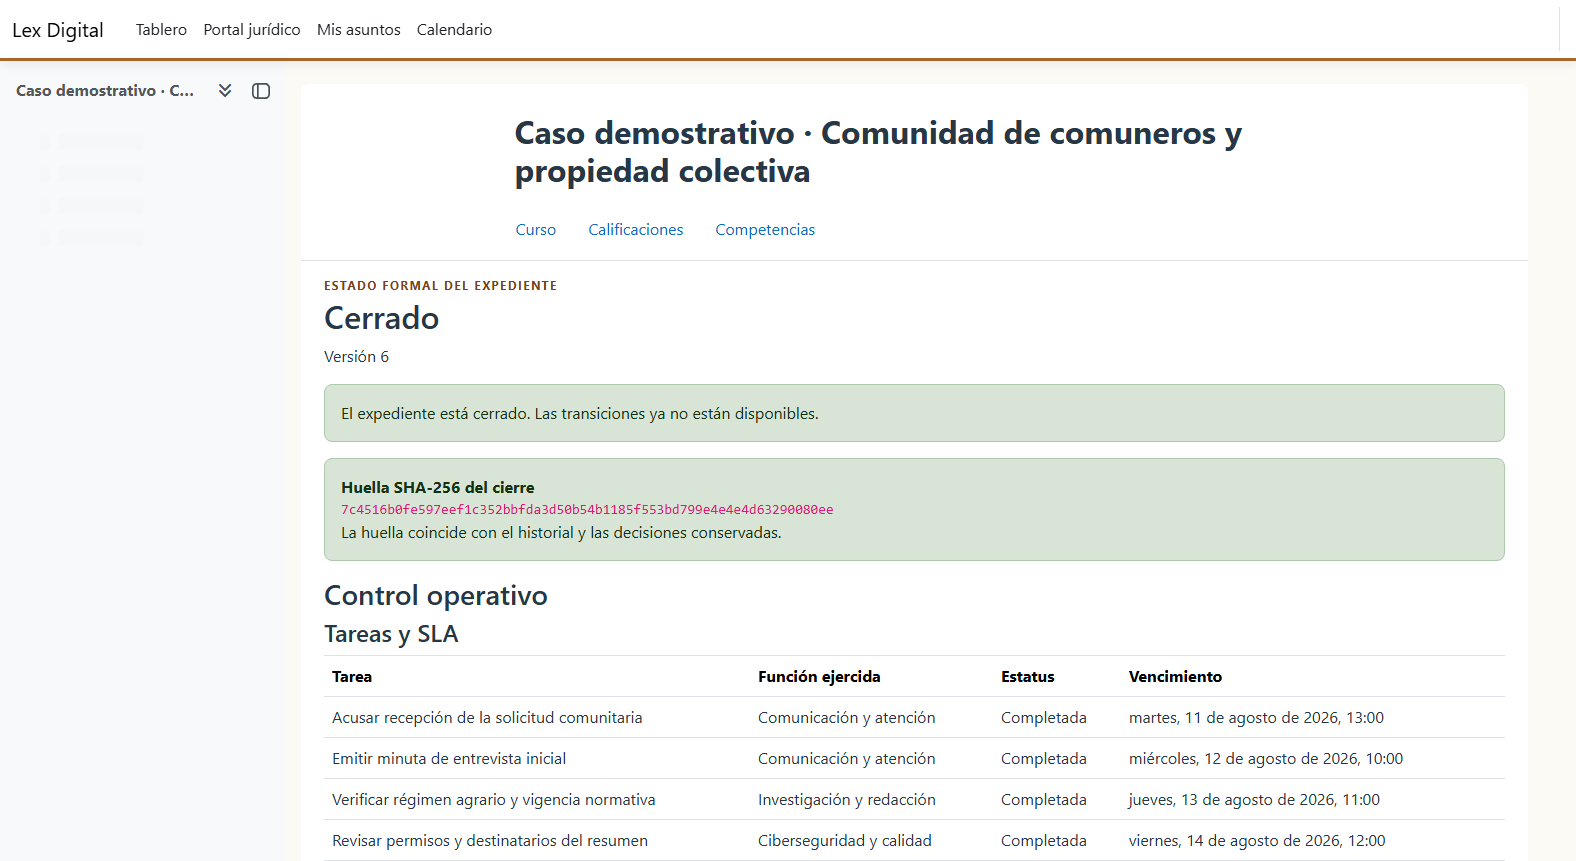
\includegraphics[width=\linewidth,height=.62\textheight,keepaspectratio]{img/actividad-7/lexdigital/03-caso-demostrativo.png}
\column{.40\textwidth}
\scriptsize
\begin{tabularx}{\linewidth}{>{\bfseries}p{1.9cm}X}
\toprule
Canal & Acuerdo de servicio \\
\midrule
Portal & Expediente, documentos y seguimiento. \\
Correo & Acuse y siguiente paso en 1 día hábil. \\
Reunión & Agenda previa y minuta el mismo día. \\
Urgencia & Aviso directo; acuse en 4 horas hábiles. \\
Bitácora & Fecha, acuerdo, responsable y plazo. \\
\bottomrule
\end{tabularx}
\vspace{3pt}
El canal se adapta a lengua, accesibilidad y conectividad; no se impone la plataforma como única vía \cite{pech2016manual,oit1691989,leyDerechosLinguisticos2024}.
\end{columns}
\vfill
{\scriptsize Ejemplo ficticio de acompañamiento a una comunidad; no acredita representación jurídica.}
\end{frame}

\begin{frame}{Trazabilidad que genera confianza}
\begin{columns}[T,onlytextwidth]
\column{.65\textwidth}
\centering
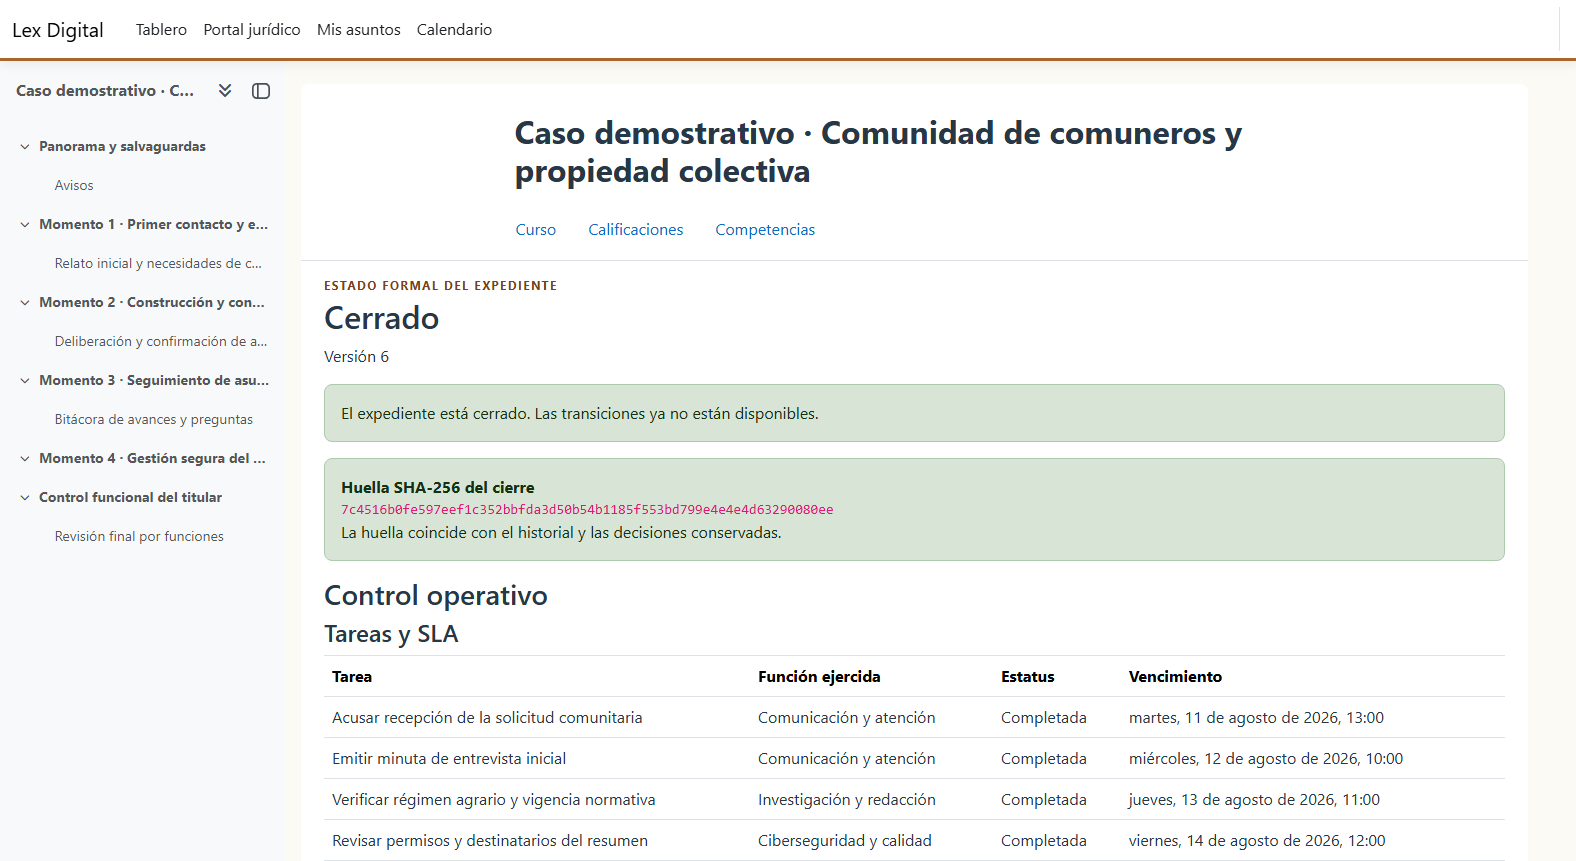
\includegraphics[width=\linewidth,height=.61\textheight,keepaspectratio]{img/actividad-7/lexdigital/04-workflow-cerrado.png}
\column{.32\textwidth}
\footnotesize
\begin{block}{La persona usuaria obtiene}
\begin{itemize}
  \item estado comprensible;
  \item consentimientos separados;
  \item acuerdos y versiones;
  \item revisión antes de entregar;
  \item cierre documentado.
\end{itemize}
\end{block}
La trazabilidad reconstruye el proceso; no es firma electrónica ni garantiza un resultado jurídico.
\end{columns}
\vfill
{\scriptsize Expediente ficticio cerrado, sin datos personales reales.}
\end{frame}

\begin{frame}{Control operativo y siguiente fase}
\begin{columns}[T,onlytextwidth]
\column{.39\textwidth}
\centering
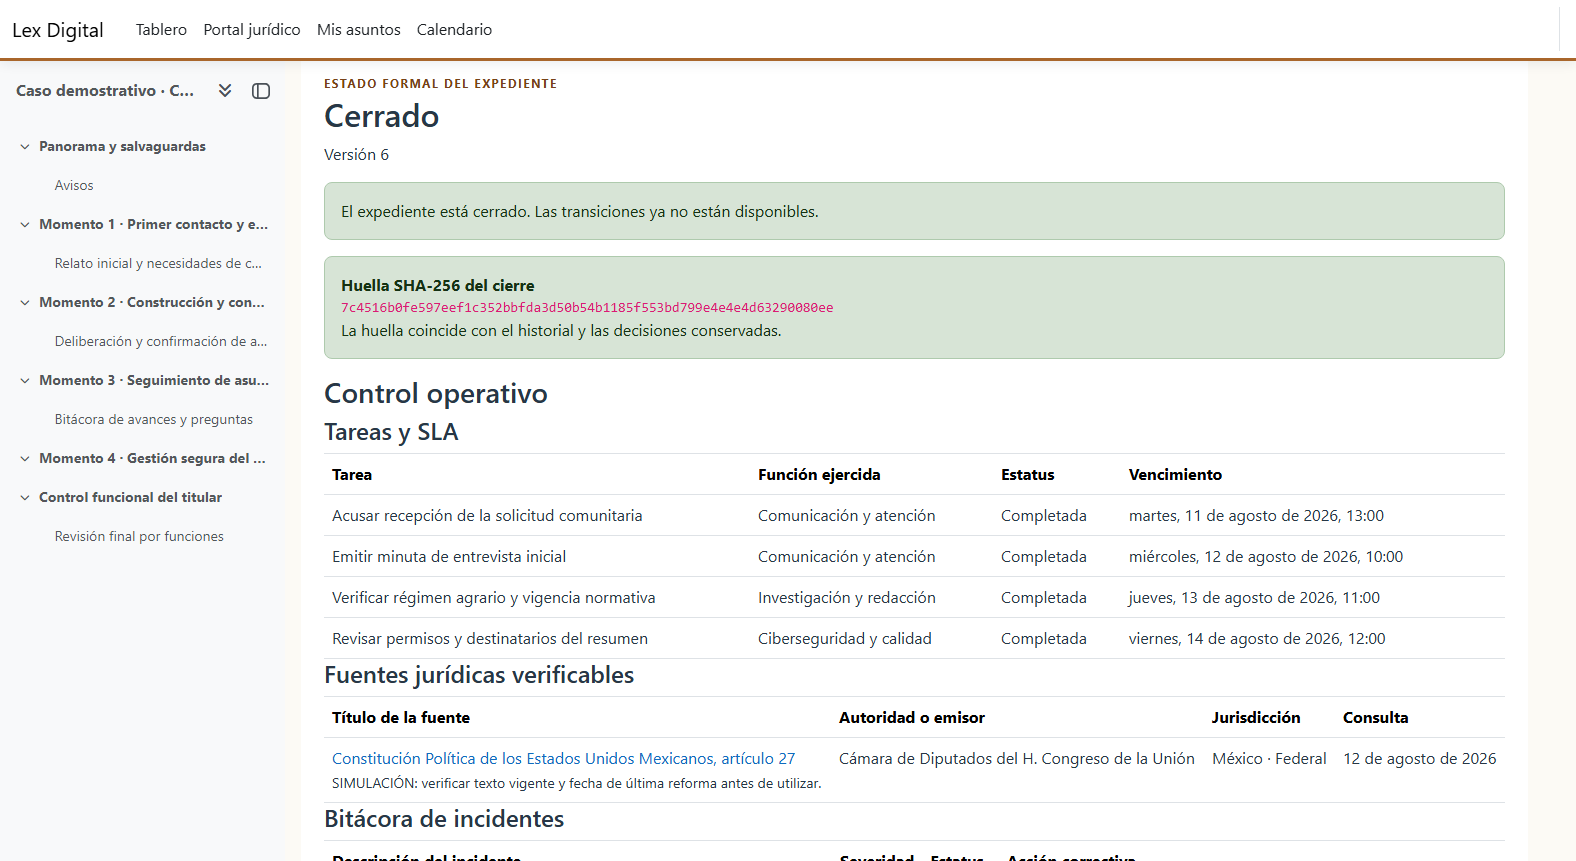
\includegraphics[width=\linewidth,height=.52\textheight,keepaspectratio]{img/actividad-7/lexdigital/05-tareas-sla.png}\\[2pt]
{\scriptsize Tareas, responsables y vencimientos}
\column{.39\textwidth}
\centering
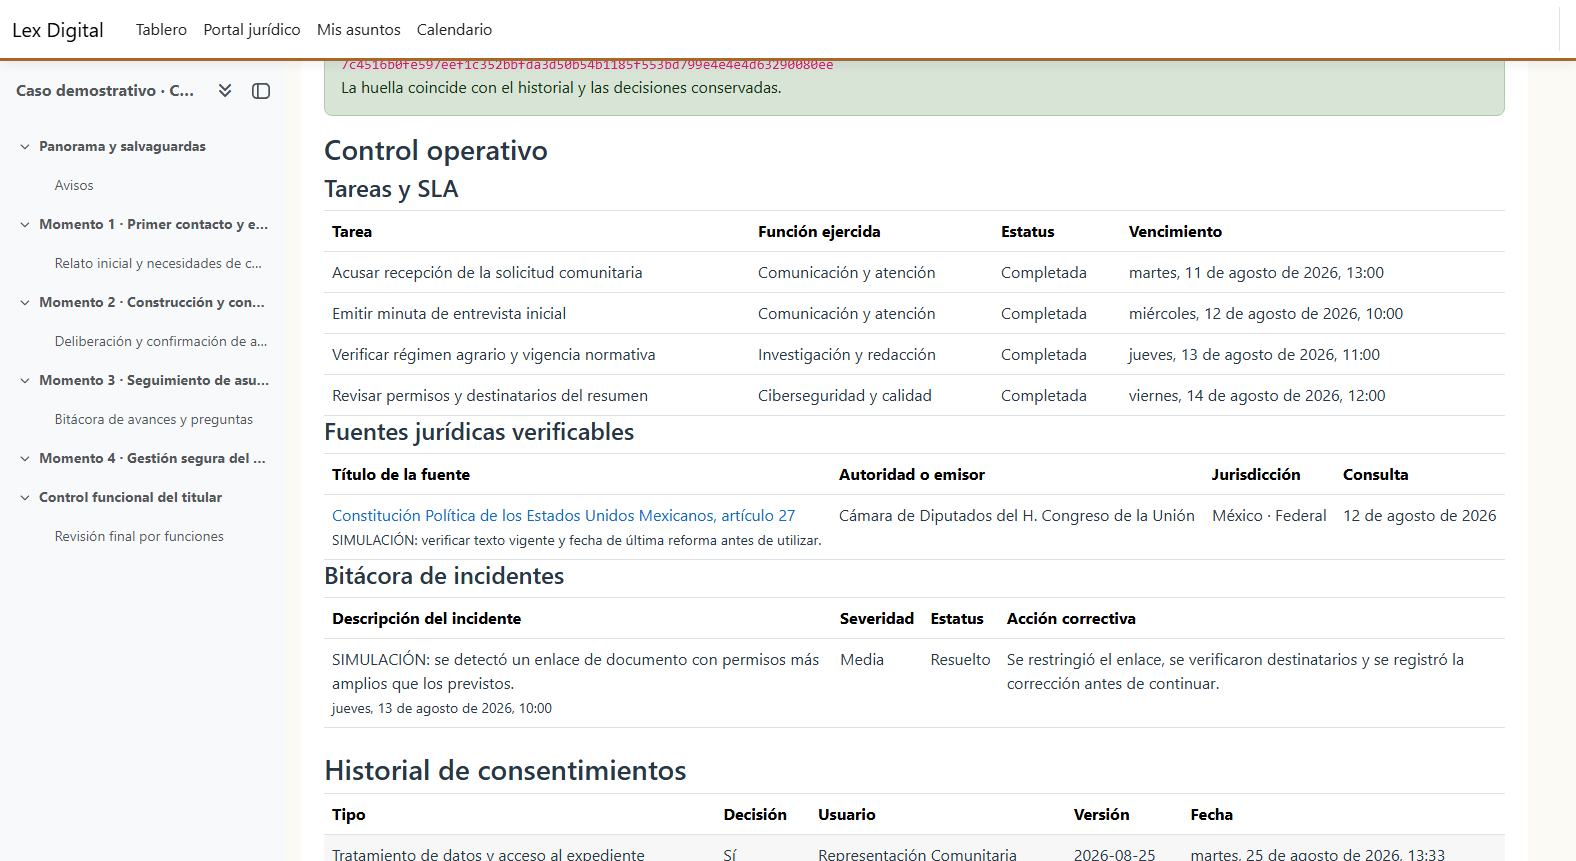
\includegraphics[width=\linewidth,height=.52\textheight,keepaspectratio]{img/actividad-7/lexdigital/06-fuentes-incidentes.png}\\[2pt]
{\scriptsize Fuentes e incidentes documentados}
\column{.19\textwidth}
\scriptsize
\begin{block}{Disponible}
Tareas, fuentes e incidentes en un caso ficticio.
\end{block}
\begin{alertblock}{Siguiente fase}
HTTPS, MFA, aviso de privacidad y pruebas integrales.
\end{alertblock}
\end{columns}
\vspace{2pt}
\begin{block}{Acceso demo para revisión docente}
\footnotesize
\href{http://54.198.73.173:8080/login/index.php}{\textbf{Ingresar al sitio | Lex Digital}}\hfill
\textbf{Usuario:} \texttt{revision.docente}\hfill
\textbf{Contraseña:} \texttt{LexA7-Revision-2026!}

\scriptsize Cuenta demostrativa de solo lectura, limitada al caso ficticio; sin edición ni administración. No deben introducirse datos reales mientras el portal use HTTP.
\end{block}
\end{frame}

\begin{frame}{Fuentes, transparencia y cierre}
\scriptsize
\begin{columns}[T,onlytextwidth]
\column{.49\textwidth}
\textbf{Fuentes jurídicas base}
\begin{thebibliography}{9}
\bibitem{cpeum2026} Cámara de Diputados. (2026). \textit{Constitución Política de los Estados Unidos Mexicanos}.
\bibitem{camaraDiputados2025lfpdppp} Cámara de Diputados. (2025). \textit{Ley Federal de Protección de Datos Personales en Posesión de los Particulares}.
\bibitem{leyDerechosLinguisticos2024} Cámara de Diputados. (2024). \textit{Ley General de Derechos Lingüísticos de los Pueblos Indígenas}.
\bibitem{oit1691989} OIT. (1989). \textit{Convenio 169 sobre pueblos indígenas y tribales}.
\bibitem{pech2016manual} Pech Salvador, C. E., Rizo García, M. y Romeu Aldaya, V. (2016). \textit{Manual de comunicación intercultural} (2.ª ed.). UACM.
\end{thebibliography}
\column{.48\textwidth}
\textbf{Organización y soporte tecnológico}
\begin{thebibliography}{9}
\bibitem{conocer2025ec0554} CONOCER. (2025). \textit{EC0554.01: Trabajo en equipo}.
\bibitem{lopezMartinez2022trabajoCooperativo} López Martínez, A. (2022). Trabajo cooperativo. En \textit{100 técnicas didácticas}. UnADM.
\bibitem{zambranoPilay2020tecnologias} Zambrano-Pilay, E. et al. (2020). Tecnologías educativas para el interaprendizaje. \textit{Yachasun, 4}(7), 200--216.
\bibitem{lexDigital2026} De la Cruz, M. J. (2026). \textit{Lex Digital: documentación del prototipo alfa 0.5.0}.
\end{thebibliography}
\end{columns}
\vspace{2pt}
\begin{block}{Compromiso}
\small Lex Digital busca convertir cada interacción jurídica digital en un proceso \textbf{comprensible, protegido y verificable}, sin prometer resultados y con revisión profesional.
\end{block}
{\scriptsize\textbf{Uso de IA:} apoyo para organizar y revisar la presentación. El portal no integra actualmente un modelo de IA; cualquier uso futuro exigirá confidencialidad, trazabilidad y revisión humana.}
\end{frame}

\end{document}
